\documentclass{beamer}

\usepackage{ucs}
\usepackage[utf8x]{inputenc}
\usepackage[T1]{fontenc}
\usepackage[english]{babel}
\usepackage{epstopdf}

\usepackage{enumitem}
\usepackage{relsize}%	relative font sizes
\usepackage{multicol}
\usepackage{todonotes}
\usepackage{xspace}
\newcommand{\computeflux}{\texttt{compute\_flux}\xspace}
\newcommand{\update}{\texttt{update}\xspace}
\newcommand{\polu}{\texttt{polu}\xspace}
\newcommand{\dirichlet}{\textit{Dirichlet}\xspace}

\graphicspath{{images/}}


%	presentation info
\title[A Finite Volume Case Study]{A Finite Volume Case Study From An Industrial Application}

\author[M. Palhas \and P. Costa]{Miguel~Palhas \and Pedro~Costa}

\institute[19808 \and 19830]{
	Department of Informatics\\
	University of Minho
}

\date{Braga, June 2012}


%	beamer options
\usetheme{CambridgeUS}

\begin{document}%	begin presentation

\frame[plain]{\titlepage}

\frame{\frametitle{Index}\tableofcontents}

\section{Case Study}

\begin{frame}[plain]
	\frametitle{\polu}
	\begin{figure}
		\centering
			\includegraphics[width=.6\textwidth]{images/foz_msh.png}
	\end{figure}
	\pause
	\begin{description}
		\item [\computeflux] computes the flux transfered through the edges;
		\item [\update] uses the compute fluxes to update the value in each cell;
	\end{description}
\end{frame}

\begin{frame}
	\frametitle{Environmental Setup}

	\begin{block}{SeARCH Group Hex}
		\begin{description}
			\item [] Intel\textsuperscript{\textregistered} Xeon\textsuperscript{\textregistered} X5650
			\item [2] processors per node;
			\item [6] cores per processor;
			\item [-] Intel\textsuperscript{\textregistered} Hyper-Threading Technology;
			\item [2.66] GHz clock frequency;
			\item [12 to 48] GB of RAM;
			\item [Tesla M2070]
			\begin{description}
				\item [1] Tesla CPU;
				\item [448] CUDA cores;
				% \item [1.15] GHz clock frequency;
				\item [515] Gflops peak (double);
				\item [6] GB dedicated memory;
				\item [148] GB/sec memory bandwidth;
			\end{description}
		\end{description}
	\end{block}
\end{frame}

\begin{frame}{Methodology}
	\begin{itemize}
		\vfill
		\item Limited execution: 5000 iterations;
		\vfill
		\item Median of 10 executions;
		\vfill
		\item 62 MB test case;
		\vfill
		\item Measurements focused on final speedups;
		\vfill
	\end{itemize}
\end{frame}

\section{Sequential}

\begin{frame}
	\begin{itemize}
		\item Initially implemented as \textbf{\itshape Arrays-of-Pointers};
		\item Accepted simplifications:
		\begin{itemize}
			\item Animation not required for program correctness;
			\item Constant velocity vectors;
		\end{itemize}
		\item Optimizations performed:
		\begin{itemize}
			\item \textbf{\itshape Arrays-Of-Structs};
			\item \textbf{\itshape Structs-Of-Arrays};
		\end{itemize}
		\item Dependencies:
		\begin{description}
			\item[\computeflux] $\Delta t$;
			\item[\update] Race condition adding edge contributions;
		\end{description}
	\end{itemize}
\end{frame}
\section{Shared Memory}

\frame{\frametitle{Index}\tableofcontents[currentsection]}

\begin{frame}
	\frametitle{OpenMP}
	\begin{block}{Implementation}
		\begin{itemize}
			\item AOS \& SOA;
			\item Similar to sequential version:
			\begin{itemize}
				\item \texttt{parallel for} added to both core functions;
			\end{itemize}
		\end{itemize}
	\end{block}

	\begin{block}{Load Balance}
		\begin{itemize}
			\item Core functions are homogeneous;
			\begin{itemize}
				\item [] (exception: \update, if number of edges per cell differs)
			\end{itemize}
			\item Static scheduling:
			\begin{itemize}
				\item Round-robin;
			\end{itemize}
		\end{itemize}
	\end{block}
\end{frame}

\begin{frame}
	\frametitle{Limitations}
	\begin{itemize}
		\vfill
		\item Locality issues:
		\vfill
		\begin{itemize}
			\item Softened with SOA;
			\vfill
			\item Depends on the mesh structure;
			\begin{itemize}
				\item \texttt{gmsh} does not optimize the mesh;
			\end{itemize}
			\vfill
			\item Highly researched topic:
			\begin{itemize}
				\item Hoppe, 1999;
				\item Complex approach;
			\end{itemize}
			\vfill
			\item Specialized libraries:
			\begin{itemize}
				\item \texttt{parmetis};
				\item Unknown complexity;
			\end{itemize}
		\end{itemize}
	\end{itemize}
\end{frame}
\section{Distributed Memory}

\frame{\frametitle{Index}\tableofcontents[currentsection,subsectionstyle=show/show/shaded]}

\subsection{Partitioning}

\begin{frame}
	\frametitle{Distributed Memory: Mesh Partitioning}

	Mesh needs to be split between each processing unit.
	\begin{block}{Ideal partitioning method:}
		\begin{enumerate}
			\item Divide the mesh into $P$ partitions;
			\item Achieve good balance between partition sizes;
			\item Keep neighbourhood information;
			\item Minimize border between them, without compromising (2).
			\item Low partitioning overhead
		\end{enumerate}
	\end{block}

\end{frame}

\subsection{Implementation}

\begin{frame}
	\frametitle{Distributed Memory: Implementation}

	Division of the mesh based only on $x$ coordinate of cells:
	\begin{enumerate}
		\item Create ordered set of cells (key is $x$ coord)
		\item Sequentially assing $N/P$ cells to each process.
	\end{enumerate}

	\begin{multicols}{2}
		\begin{figure}
			\begin{center}
				\includegraphics[width=0.955\columnwidth]{foz_msh}
			\end{center}
		\end{figure}
		\pause
		\begin{figure}
			\begin{center}
				\includegraphics[width=0.955\columnwidth]{foz_p4_msh}
			\end{center}
		\end{figure}
	\end{multicols}
\end{frame}

\begin{frame}
	\frametitle{Distributed Memory: Implementation}

	\begin{block}{Two step communication}
		\begin{itemize}\itemsep=20pt
			\item Performed in two steps:
			\begin{enumerate}\itemsep=10pt
				\item Send to left / Receive from right
				\item Send to right / Receive from left
			\end{enumerate}

			\item Not homogeneous (no control over border size)

			\item Only 2 processes per node use the network
			\begin{itemize}
				\item Assuming best process asignement is used
			\end{itemize}
		\end{itemize}
	\end{block}
\end{frame}

\begin{frame}
\frametitle{Distributed Memory: Implementation}

	\begin{block}{Advantages}
		\begin{enumerate}\itemsep=10pt
			\item Simple concept and implementation
			\item Each partition has a left and a right neighbour
			\begin{itemize}
				\item[-] Communication in two steps only
			\end{itemize}
		\end{enumerate}
	\end{block}

	\begin{block}{Disadvantages}
		\begin{enumerate}\itemsep=10pt
			\item No control over size of border between partitions (communication)
			\item Sequential sort and distribution are slow
		\end{enumerate}
	\end{block}

\end{frame}

\begin{frame}
	\frametitle{Results}
	\begin{figure}
		\centering
		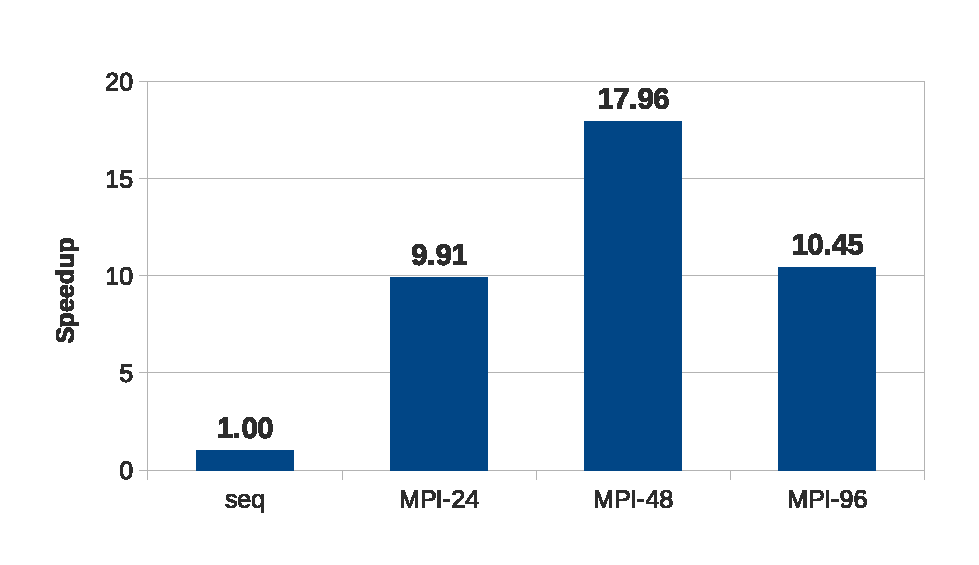
\includegraphics[width=0.8\textwidth]{graph_comparison_mpi.eps}
	\end{figure}
\end{frame}


\section{GPU}

\frame{\frametitle{Index}\tableofcontents[currentsection]}

%
% IMPLEMENTATION
%
\frame{\frametitle{GPU}

	\begin{block}{Implementation}
		\begin{itemize}\itemsep=20pt
			\item \textit{Struct-of-Arrays}
			\pause

			\item \texttt{compute\_flux} and \texttt{update} directly converted to CUDA Kernels
			\begin{itemize}
				\item[-] Each iteration mapped to one CUDA Thread
			\end{itemize}
			\pause

			\item One aditional \texttt{reduction} kernel (later removed)
			\pause

			\item Data transfers only happen before the main loop
			\pause
			\begin{itemize}
				\item[] (exception: animation output, which is removed)
			\end{itemize}
		\end{itemize}
	\end{block}
}

\frame{\frametitle{GPU}
	\begin{block}{Load Balance}
		\begin{itemize}\itemsep=20pt
			\item workload of both kernels is homogeneous
			\pause
			\begin{itemize}
				\item[] (exception: for \update kernel, if number of edges per cell differs)
			\end{itemize}
			\pause
		\end{itemize}
	\end{block}

	\begin{block}{Limitations}
		\begin{itemize}
			\item Memory accesses are the main issue
			\pause
			\begin{itemize}
				\item[-] \computeflux will not access cells in order
				\item[-] Same problem for \update when accessing edges
			\end{itemize}

		\end{itemize}
	\end{block}
}


% \section{Experiment}

\frame{\frametitle{Index}\tableofcontents[currentsection,subsectionstyle=show/show/shaded]}

\begin{frame}
	\frametitle{Environmental Setup}

	\begin{block}{SeARCH Group Hex}
		\begin{description}
			\item [] Intel\textsuperscript{\textregistered} Xeon\textsuperscript{\textregistered} X5650
			\item [2] processors per node;
			\item [6] cores per processor;
			\item [-] Intel\textsuperscript{\textregistered} HyperThreading Technology;
			\item [2.66] GHz clock frequency;
			\item [12 to 48] GB of RAM;
			\item [Tesla C2070]
			\begin{description}
				\item [1] Tesla CPU;
				\item [448] CUDA cores;
				\item [1.15] GHz clock frequency;
				\item [515] Gflops peak (double);
				\item [6] GB dedicated memory;
				\item [144] GB/sec memory bandwidth;
			\end{description}
		\end{description}
	\end{block}
\end{frame}

\begin{frame}{Methodology}
	\begin{itemize}
		\vfill
		\item Limited execution: 5000 iterations;
		\vfill
		\item Median of 10 executions;
		\vfill
		\item 62 MB test case;
		\vfill
		\item Measurements focused on final speedups;
		\vfill
	\end{itemize}
\end{frame}

\begin{frame}
	\frametitle{Speedups}
	\begin{figure}
		\centering
		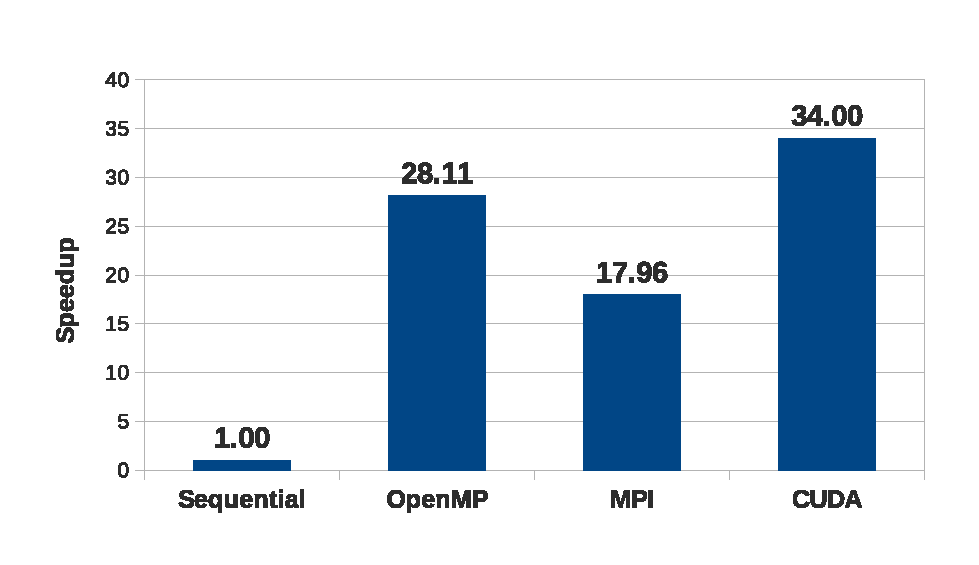
\includegraphics[width=0.8\textwidth]{graph_comparison_all.eps}
	\end{figure}
\end{frame}

% \input{slides/70-conclusion}

\begin{frame}[plain]
	\titlepage
	\begin{center}
		\Huge\bfseries - ? -
	\end{center}
\end{frame}

\end{document}%	end presentation
